\documentclass{standalone}
\usepackage{tikz}
\usetikzlibrary{patterns, positioning}


\begin{document}
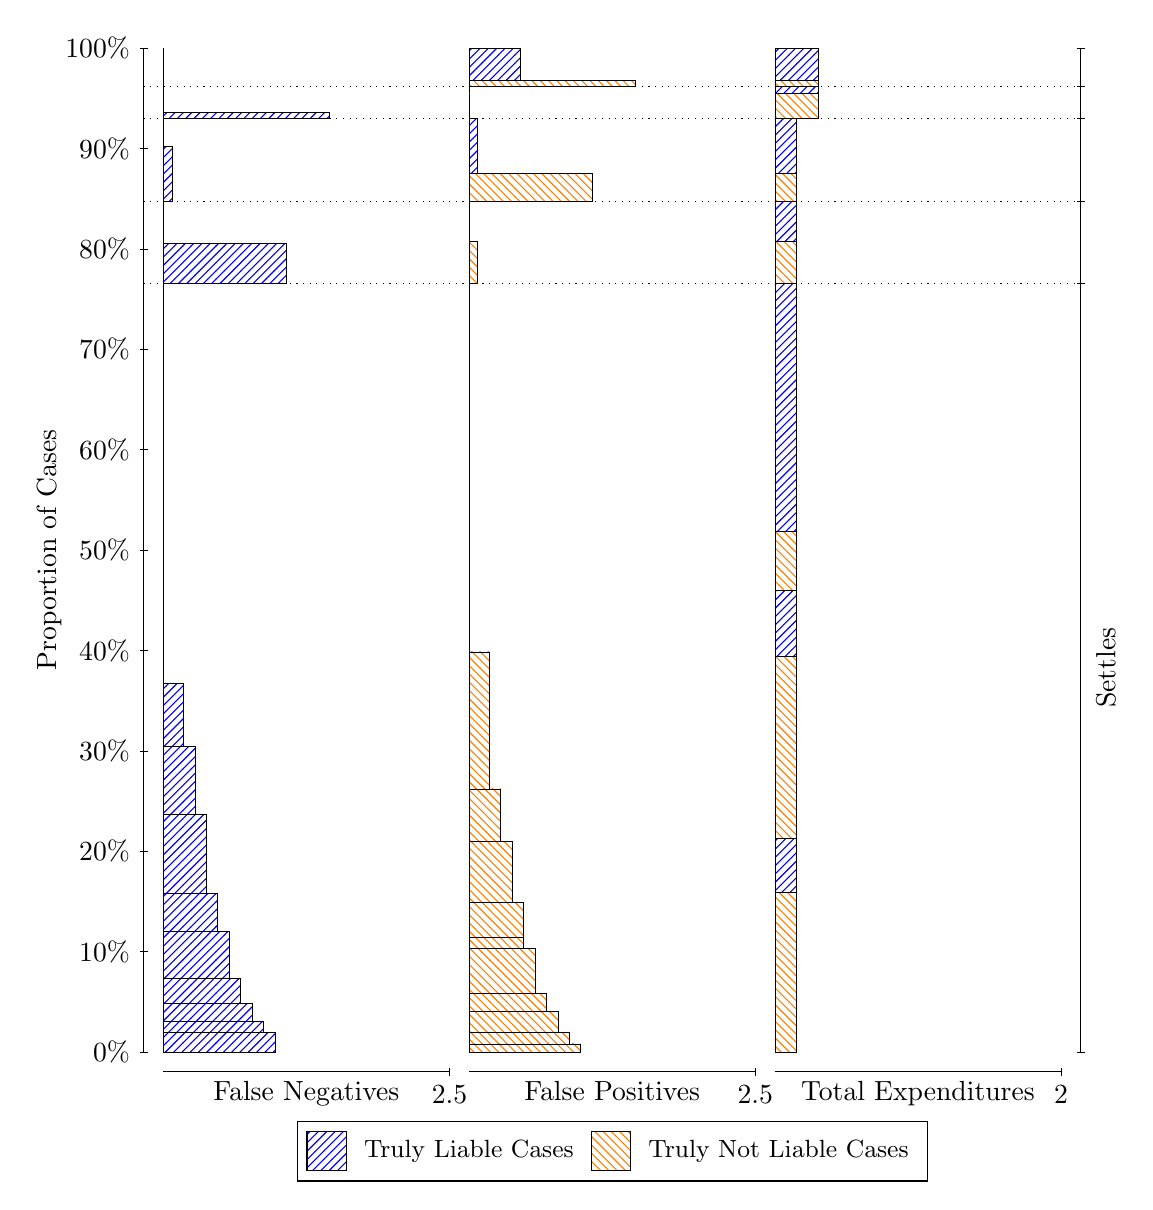
\begin{tikzpicture}
\draw[black, very thin] (1.5,1.75) -- (1.5,14.5);
\node[rotate=90, text=black, anchor=center] at (0.3, 8.125) {Proportion of Cases};
\draw[black, very thin] (1.45,1.75) -- (1.55,1.75);
\node[text=black, anchor=east] at (1.45, 1.75) {0\%};
\draw[black, very thin] (1.45,3.025) -- (1.55,3.025);
\node[text=black, anchor=east] at (1.45, 3.025) {10\%};
\draw[black, very thin] (1.45,4.3) -- (1.55,4.3);
\node[text=black, anchor=east] at (1.45, 4.3) {20\%};
\draw[black, very thin] (1.45,5.575) -- (1.55,5.575);
\node[text=black, anchor=east] at (1.45, 5.575) {30\%};
\draw[black, very thin] (1.45,6.85) -- (1.55,6.85);
\node[text=black, anchor=east] at (1.45, 6.85) {40\%};
\draw[black, very thin] (1.45,8.125) -- (1.55,8.125);
\node[text=black, anchor=east] at (1.45, 8.125) {50\%};
\draw[black, very thin] (1.45,9.4) -- (1.55,9.4);
\node[text=black, anchor=east] at (1.45, 9.4) {60\%};
\draw[black, very thin] (1.45,10.675) -- (1.55,10.675);
\node[text=black, anchor=east] at (1.45, 10.675) {70\%};
\draw[black, very thin] (1.45,11.95) -- (1.55,11.95);
\node[text=black, anchor=east] at (1.45, 11.95) {80\%};
\draw[black, very thin] (1.45,13.225) -- (1.55,13.225);
\node[text=black, anchor=east] at (1.45, 13.225) {90\%};
\draw[black, very thin] (1.45,14.5) -- (1.55,14.5);
\node[text=black, anchor=east] at (1.45, 14.5) {100\%};

\draw[black, very thin] (13.4,1.75) -- (13.4,14.5);
\draw[black, very thin] (13.35,1.75) -- (13.45,1.75);
\node[anchor=west] at (13.35, 1.75) {};
\draw[black, very thin] (13.35,11.508) -- (13.45,11.508);
\node[anchor=west] at (13.35, 11.508) {};
\draw[black, very thin] (13.35,12.548) -- (13.45,12.548);
\node[anchor=west] at (13.35, 12.548) {};
\draw[black, very thin] (13.35,13.603) -- (13.45,13.603);
\node[anchor=west] at (13.35, 13.603) {};
\draw[black, very thin] (13.35,14.008) -- (13.45,14.008);
\node[anchor=west] at (13.35, 14.008) {};
\draw[black, very thin] (13.35,14.5) -- (13.45,14.5);
\node[anchor=west] at (13.35, 14.5) {};

\draw[black, very thin, pattern color=blue, pattern=north east lines] (1.75,1.75) rectangle (3.167,1.9993);
\draw[black, very thin, pattern color=blue, pattern=north east lines] (1.75,1.9993) rectangle (3.0217,2.1345);
\draw[black, very thin, pattern color=blue, pattern=north east lines] (1.75,2.1345) rectangle (2.8763,2.3685);
\draw[black, very thin, pattern color=blue, pattern=north east lines] (1.75,2.3685) rectangle (2.731,2.6824);
\draw[black, very thin, pattern color=blue, pattern=north east lines] (1.75,2.6824) rectangle (2.5857,3.2769);
\draw[black, very thin, pattern color=blue, pattern=north east lines] (1.75,3.2769) rectangle (2.4403,3.7653);
\draw[black, very thin, pattern color=blue, pattern=north east lines] (1.75,3.7653) rectangle (2.295,4.7639);
\draw[black, very thin, pattern color=blue, pattern=north east lines] (1.75,4.7639) rectangle (2.1497,5.6356);
\draw[black, very thin, pattern color=blue, pattern=north east lines] (1.75,5.6356) rectangle (2.0043,6.4273);
\draw[black, very thin, pattern color=orange, pattern=north west lines] (1.75,6.4273) rectangle (1.75,11.508);
\draw[black, very thin, pattern color=blue, pattern=north east lines] (1.75,11.508) rectangle (3.3123,12.015);
\draw[black, very thin, pattern color=orange, pattern=north west lines] (1.75,12.015) rectangle (1.75,12.548);
\draw[black, very thin, pattern color=blue, pattern=north east lines] (1.75,12.548) rectangle (1.859,13.247);
\draw[black, very thin, pattern color=orange, pattern=north west lines] (1.75,13.247) rectangle (1.75,13.603);
\draw[black, very thin, pattern color=blue, pattern=north east lines] (1.75,13.603) rectangle (3.8573,13.687);
\draw[black, very thin, pattern color=orange, pattern=north west lines] (1.75,13.687) rectangle (1.75,14.008);
\draw[black, very thin, pattern color=orange, pattern=north west lines] (1.75,14.008) rectangle (1.75,14.092);
\draw[black, very thin, pattern color=blue, pattern=north east lines] (1.75,14.092) rectangle (1.75,14.5);
\draw[black, very thin, pattern color=orange, pattern=north west lines] (5.6333,1.75) rectangle (7.0503,1.853);
\draw[black, very thin, pattern color=orange, pattern=north west lines] (5.6333,1.853) rectangle (6.905,1.9994);
\draw[black, very thin, pattern color=orange, pattern=north west lines] (5.6333,1.9994) rectangle (6.7597,2.2639);
\draw[black, very thin, pattern color=orange, pattern=north west lines] (5.6333,2.2639) rectangle (6.6143,2.4938);
\draw[black, very thin, pattern color=orange, pattern=north west lines] (5.6333,2.4938) rectangle (6.469,3.0607);
\draw[black, very thin, pattern color=orange, pattern=north west lines] (5.6333,3.0607) rectangle (6.3237,3.2073);
\draw[black, very thin, pattern color=orange, pattern=north west lines] (5.6333,3.2073) rectangle (6.3237,3.6466);
\draw[black, very thin, pattern color=orange, pattern=north west lines] (5.6333,3.6466) rectangle (6.1783,4.4225);
\draw[black, very thin, pattern color=orange, pattern=north west lines] (5.6333,4.4225) rectangle (6.033,5.0909);
\draw[black, very thin, pattern color=orange, pattern=north west lines] (5.6333,5.0909) rectangle (5.8877,6.8304);
\draw[black, very thin, pattern color=blue, pattern=north east lines] (5.6333,6.8304) rectangle (5.6333,11.508);
\draw[black, very thin, pattern color=orange, pattern=north west lines] (5.6333,11.508) rectangle (5.7423,12.041);
\draw[black, very thin, pattern color=blue, pattern=north east lines] (5.6333,12.041) rectangle (5.6333,12.548);
\draw[black, very thin, pattern color=orange, pattern=north west lines] (5.6333,12.548) rectangle (7.1957,12.905);
\draw[black, very thin, pattern color=blue, pattern=north east lines] (5.6333,12.905) rectangle (5.7423,13.603);
\draw[black, very thin, pattern color=orange, pattern=north west lines] (5.6333,13.603) rectangle (5.6333,13.925);
\draw[black, very thin, pattern color=blue, pattern=north east lines] (5.6333,13.925) rectangle (5.6333,14.008);
\draw[black, very thin, pattern color=orange, pattern=north west lines] (5.6333,14.008) rectangle (7.7407,14.092);
\draw[black, very thin, pattern color=blue, pattern=north east lines] (5.6333,14.092) rectangle (6.2873,14.5);
\draw[black, very thin, pattern color=orange, pattern=north west lines] (9.5167,1.75) rectangle (9.7892,3.7802);
\draw[black, very thin, pattern color=blue, pattern=north east lines] (9.5167,3.7802) rectangle (9.7892,4.4633);
\draw[black, very thin, pattern color=orange, pattern=north west lines] (9.5167,4.4633) rectangle (9.7892,6.7697);
\draw[black, very thin, pattern color=blue, pattern=north east lines] (9.5167,6.7697) rectangle (9.7892,7.6135);
\draw[black, very thin, pattern color=orange, pattern=north west lines] (9.5167,7.6135) rectangle (9.7892,8.3573);
\draw[black, very thin, pattern color=blue, pattern=north east lines] (9.5167,8.3573) rectangle (9.7892,11.508);
\draw[black, very thin, pattern color=orange, pattern=north west lines] (9.5167,11.508) rectangle (9.7892,12.041);
\draw[black, very thin, pattern color=blue, pattern=north east lines] (9.5167,12.041) rectangle (9.7892,12.548);
\draw[black, very thin, pattern color=orange, pattern=north west lines] (9.5167,12.548) rectangle (9.7892,12.905);
\draw[black, very thin, pattern color=blue, pattern=north east lines] (9.5167,12.905) rectangle (9.7892,13.603);
\draw[black, very thin, pattern color=orange, pattern=north west lines] (9.5167,13.603) rectangle (10.062,13.925);
\draw[black, very thin, pattern color=blue, pattern=north east lines] (9.5167,13.925) rectangle (10.062,14.008);
\draw[black, very thin, pattern color=orange, pattern=north west lines] (9.5167,14.008) rectangle (10.062,14.092);
\draw[black, very thin, pattern color=blue, pattern=north east lines] (9.5167,14.092) rectangle (10.062,14.5);
\draw[black, dotted] (1.5,11.508) -- (13.4,11.508);
\draw[black, dotted] (1.5,12.548) -- (13.4,12.548);
\draw[black, dotted] (1.5,13.603) -- (13.4,13.603);
\draw[black, dotted] (1.5,14.008) -- (13.4,14.008);
\draw[black, very thin] (1.75,1.5) -- (5.3833,1.5);
\node[text=black, anchor=north] at (3.5667, 1.5) {False Negatives};
\draw[black, very thin] (5.3833,1.45) -- (5.3833,1.55);
\node[text=black, anchor=north] at (5.3833, 1.45) {2.5};

\draw[black, very thin] (5.6333,1.5) -- (9.2667,1.5);
\node[text=black, anchor=north] at (7.45, 1.5) {False Positives};
\draw[black, very thin] (9.2667,1.45) -- (9.2667,1.55);
\node[text=black, anchor=north] at (9.2667, 1.45) {2.5};

\draw[black, very thin] (9.5167,1.5) -- (13.15,1.5);
\node[text=black, anchor=north] at (11.333, 1.5) {Total Expenditures};
\draw[black, very thin] (13.15,1.45) -- (13.15,1.55);
\node[text=black, anchor=north] at (13.15, 1.45) {2};

\node[text=black, centered, rotate=90] at (13.72, 6.6289) {Settles};





\draw (7.449999999999999,1.5) node[draw=none] (baseCoordinate) {};
\begin{scope}[align=center]
        \matrix[scale=0.5, draw=black, below=0.5cm of baseCoordinate, nodes={draw}, column sep=0.1cm]{
            \node[rectangle, draw, minimum width=0.5cm, minimum height=0.5cm, pattern color=blue, pattern=north east lines] {}; &
            \node[draw=none, font=\small, text=black] (B) {Truly Liable Cases}; &
            \node[rectangle, draw, minimum width=0.5cm, minimum height=0.5cm, pattern color=orange, pattern=north west lines] {}; &
            \node[draw=none, font=\small, text=black] (B) {Truly Not Liable Cases}; \\
            };
\end{scope}

\end{tikzpicture}
\end{document}